\section{Evaluation}
\label{sec:eval}
We will evaluate our system on the metrics of performance, 
availability and scalability. To measure performance, 
we will design benchmarks to measure the data rate 
of a listener versus the data rate of the host. To 
evaluate availability, we will examine how our system 
behaves with various failure modes by artificially 
taking down each role (client, master server, session 
server). For scalability, we will measure system 
performance as we add clients to the system. We can 
achieve this by launching our application on an 
increasing number of client machines.

\subsection{Performance}

For the performance of our system, we are interested in
differences in playback between clients in the same session.
We want clients to be listening to not just the same song,
but the position in the song. To test this, we set up two
different experiments.

\begin{enumerate}

\item Determine differences in playback between a host and a
listener as more active sessions are added to the system.

\item Determine differences in playback between a host and a
listener as more listeners are added to their session.

\end{enumerate}

The host and listener were set up as different users on the same machine
so as to have identical clocks. The added sessions or listeners
were achieved through a modified version of Google's load test
for App Engine applications. Differences in playback were observed
through comparing the ending timestamps of songs between the host
and listener. Each experiment followed a similar series of steps,
listed below.

\begin{enumerate}

\item The host starts a session by choosing a song.

\item The listener joins the host's newly created session.

\item New sessions/listeners are added to the system.

\item The time the current song ended is recorded for both the
host and listener.

\item The host adds a new song. Go to step 3.

\end{enumerate}

The results for adding more active sessions are shown in Figure
~\ref{fig:addSessions}. As more sessions were added to the system,
there wasn't much of a difference in song playback between the host
and listener. On average the difference actually decreased as more
sessions were added, but this is likely due to the outlier observed
for 30 sessions. The minor differences observed are more likely to
have been caused by external network-related factors than by our
system itself.

\begin{figure}[h]
	\centering
	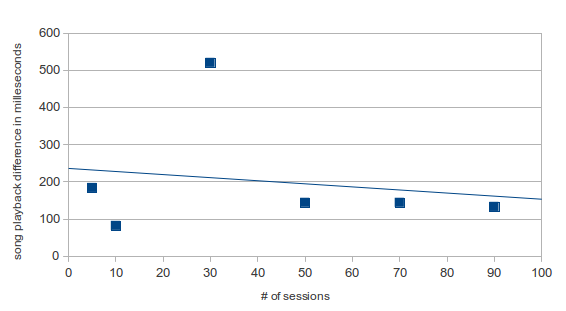
\includegraphics[width=0.5\textwidth]{add_sessions.png}
	\caption{Playback difference when adding more sessions.}
	\label{fig:addSessions}
\end{figure}

The results for adding more listeners are shown in Figure~\ref{fig:addListeners}. As more listeners were added to a
session, there was a minor increase in song playback differences
between the host and listener. However, even with 90 active listeners
in a session, the difference was less than 1 second. This increase is
likely due to the additional work the server has to perform to
propagate updates to an increasing number of listeners in the
session.

\begin{figure}[h]
	\centering
	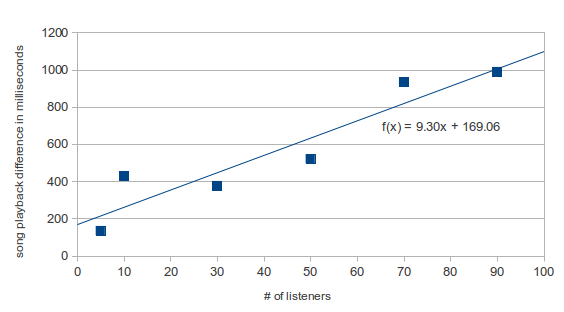
\includegraphics[width=0.5\textwidth]{add_listeners.png}
	\caption{Playback difference when adding more listeners.}
	\label{fig:addListeners}
\end{figure}

We also recorded the response time of our system as more listeners
were added to a session. The results are shown in
Figure~\ref{fig:addListenersResponseTime}. The response time
increased as more listeners were added to a session, starting at
around .5 seconds and reaching nearly 5 seconds. This is to be
expected as the server propagates session updates to all listeners
when a new listener joins a session. As more listeners join a
session, the server has to send more updates. Even with nearly
100 listeners, the response time was still under 5 seconds. This
is likely acceptable, but not ideal. To reduce this time, the serve
could propagate updates only on song changes which would reduce
its overhead at the cost of hosts having an outdated view of
session information.

\begin{figure}[h]
	\centering
	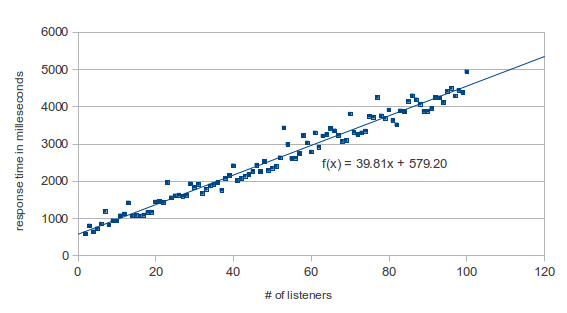
\includegraphics[width=0.5\textwidth]{add_listeners_response_time.png}
	\caption{Response time when adding more listeners.}
	\label{fig:addListenersResponseTime}
\end{figure}

\subsection{Availability}

For the availability of our system, we are interested in session
availability among failures of certain system components. There are
several components that can possibly fail including the host,
listener, session server, and master server. To evaluate the
effects of such failures, we artificially caused each role to fail
during an active session and observed the system behavior for the
host, listener, and other clients.

When the host of a session goes down, the system mainly continues
to operate as normal. Any listeners in the session of the down host
will continue playing the current song until completion. At that
time, they will wait until the host reconnects and updates the
session server with new information. Other clients will still be
able to join the session, but will have to wait like other
listeners. Once the host reconnects, it rejoins its hosted session
and continues playback as if it just joined the session.

A down listener has very little impact on the system. The session
server will detect the channel failure and cleanup necessary state
associated with the listener. Other listeners as well as the host
of the session will not be impacted by the failed listener.

When the master server goes down, active sessions continue to
operate as before. Hosts and listeners can continue to listen
together to existing and newly added songs. However, new clients
attempting to connect to the system will have their requests time
out because the master server handles all initial client connections.

If the session server goes down, all session updates will fail.
Clients will finish their current song of their session and then
will have to wait for the session server to come back up. New clients
first connecting to the system will be able to login, but will not
see any sessions. They will also be unable to start a session until
the session server comes back up.